% ============================ Part 6: Alignment ============================
\section{Part 6 $\cdot$ Alignment}

\begin{frame}{Why alignment? Predicting text is not the same as being helpful}
\begin{columns}[T]
\begin{column}{0.52\textwidth}
\begin{itemize}\setlength{\itemsep}{6pt}
  \item \textbf{Objective mismatch:} ``predict the next word'' says nothing about being helpful, truthful, or safe.
  \item \textbf{Data bias:} web text contains toxic and misleading content; the LM does not distinguish good from bad behavior.
  \item GPT-3 (2020) was impressive but awkward to use; ChatGPT (2022) = the same kind of model + \textbf{alignment}.
  \item Target --- ``HHH'': \textbf{helpful}, \textbf{honest}, \textbf{harmless}.
\end{itemize}
\end{column}
\begin{column}{0.46\textwidth}
\keybox{\textbf{How do you write a loss function for \dots}\\[4pt]
\quad what is helpful? \quad what is funny?\\
\quad what is ethical? \quad what is safe?\\[6pt]
You don't. You \textbf{learn} it from human judgments --- then optimize it with RL (Part 5).}
\end{column}
\end{columns}
\end{frame}

\begin{frame}{Step 1: collect comparisons, not scores}
\begin{columns}[T]
\begin{column}{0.5\textwidth}
\centering
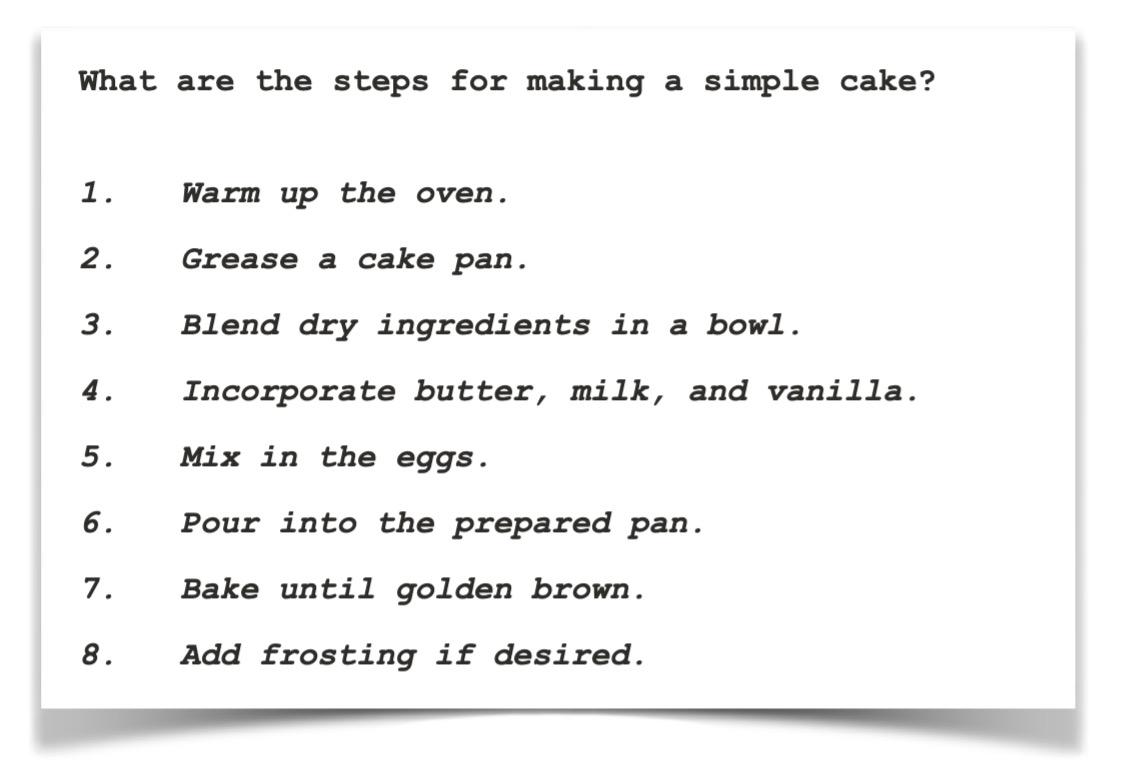
\includegraphics[width=0.72\textwidth]{figs/pref_absolute.png}\\[2pt]
\scriptsize ``Rate this answer 1--10'': different people give very different numbers for the same text.
\end{column}
\begin{column}{0.48\textwidth}
\centering
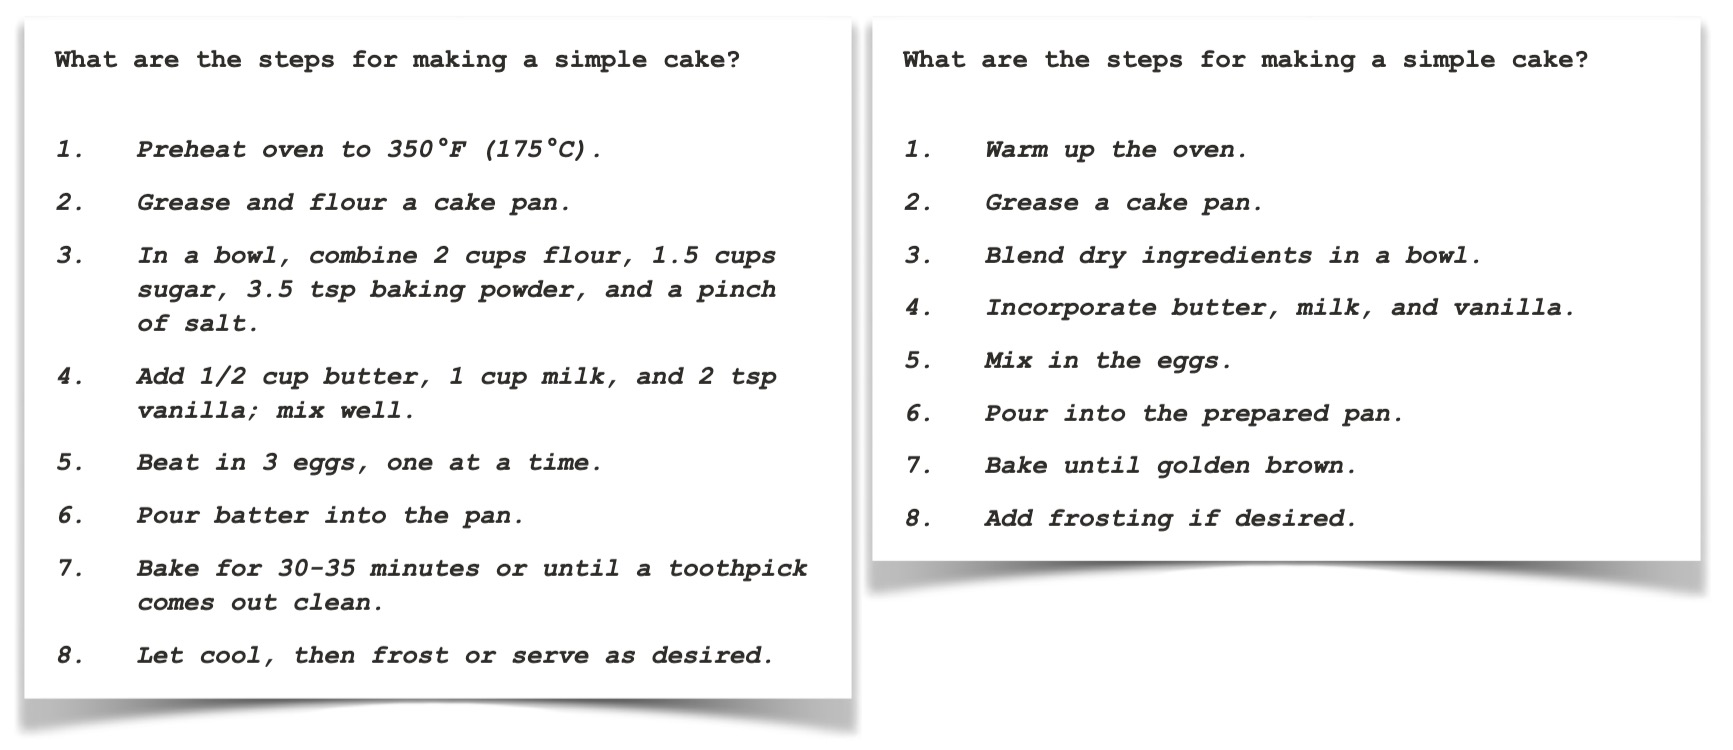
\includegraphics[width=0.95\textwidth]{figs/pref_pairs.png}\\[2pt]
\scriptsize ``Which of the two is better?'': humans are much more consistent at relative judgments.
\end{column}
\end{columns}
\vspace{8pt}
\keybox{Preference data = triples $(x,\; y_w,\; y_l)$: prompt, \textbf{w}inning response, \textbf{l}osing response, both sampled from the model.}
\end{frame}

\begin{frame}{Preference data at scale: UltraFeedback}
\begin{center}
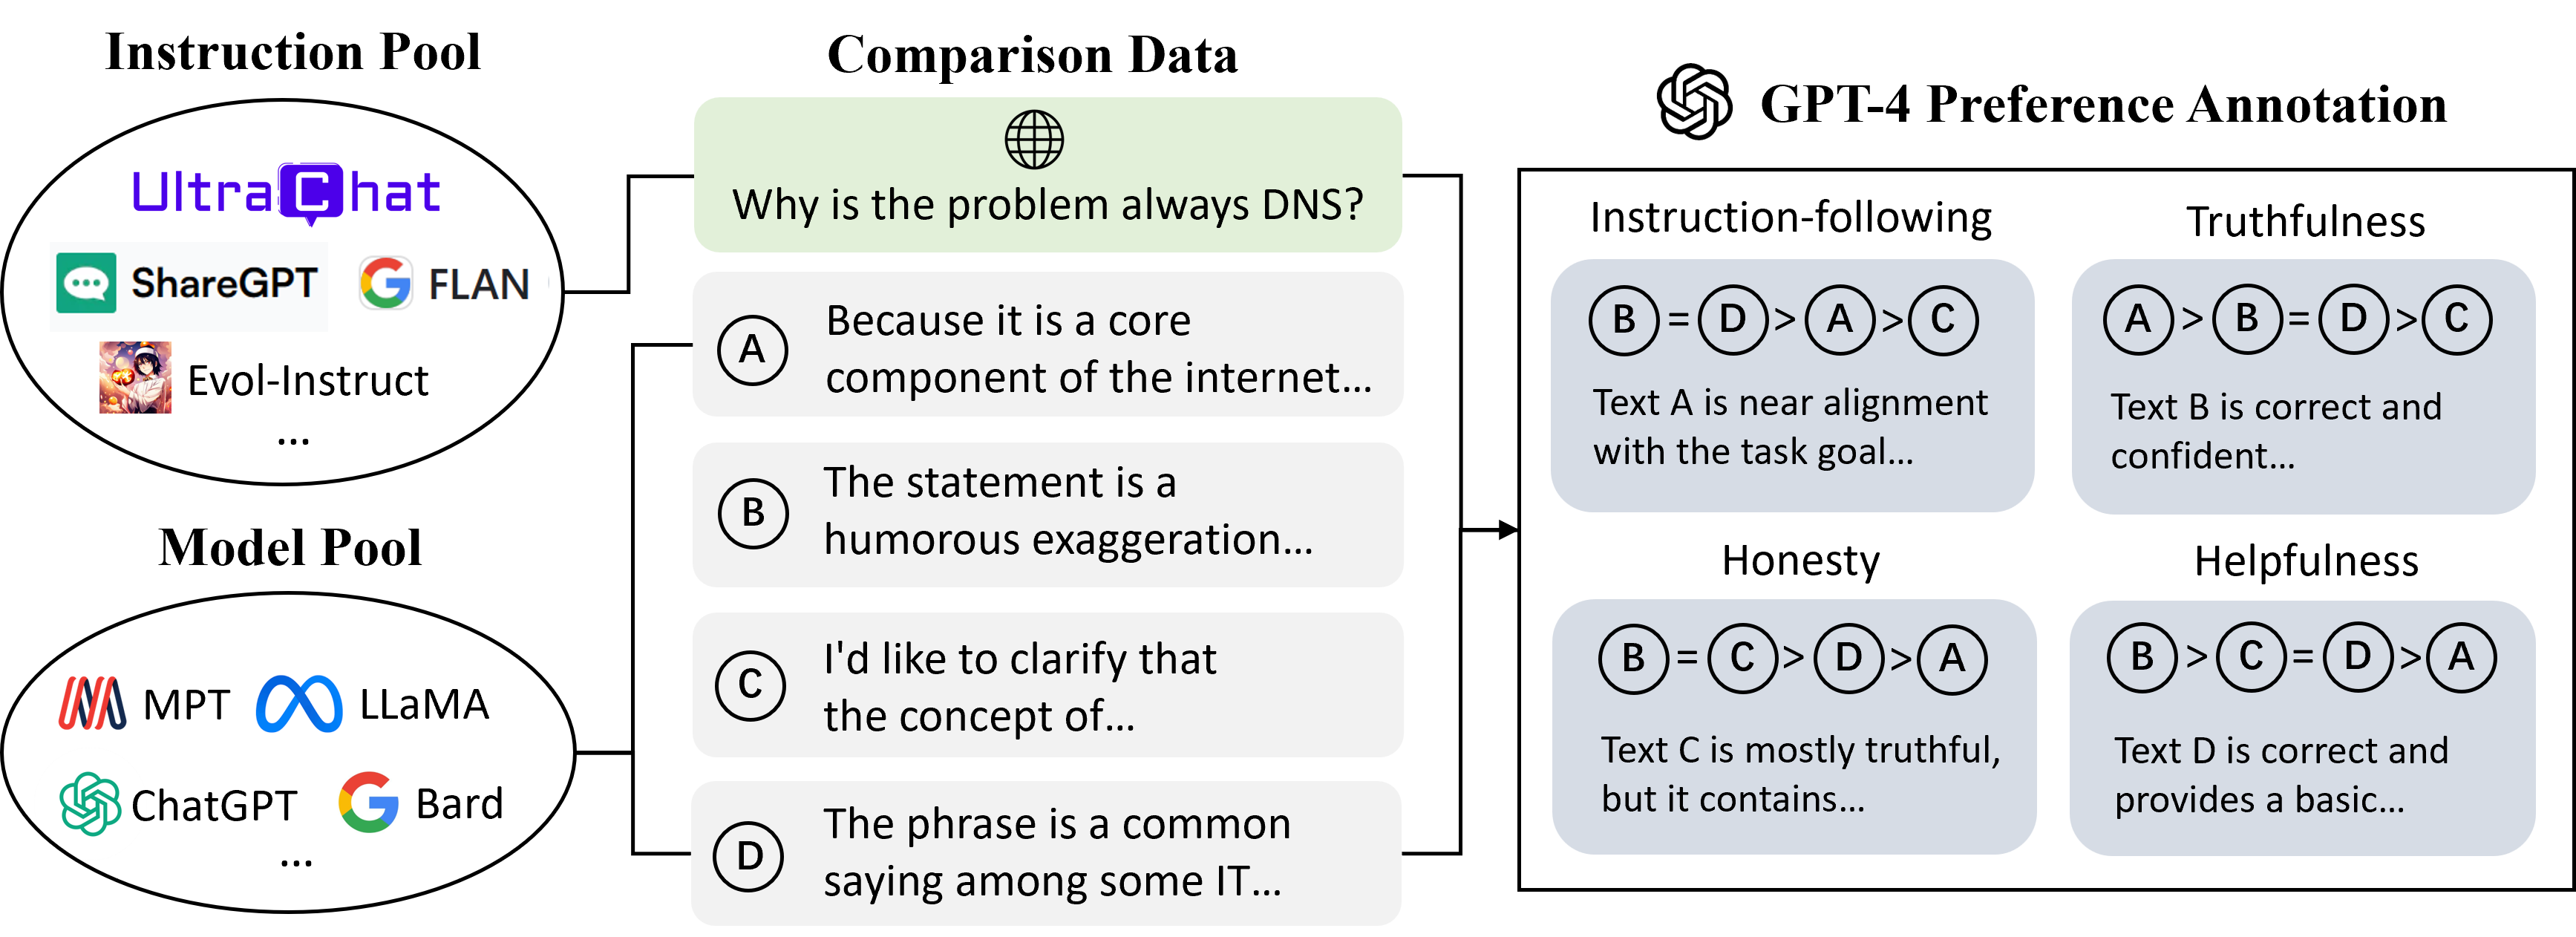
\includegraphics[width=0.95\textwidth]{figs/ultrafeedback.png}
\end{center}
\begin{itemize}\setlength{\itemsep}{4pt}
  \item 60k prompts from many instruction datasets; 4 responses per prompt from different LLMs.
  \item Each response rated by \textbf{GPT-4} on instruction-following, truthfulness, honesty, helpfulness (``RLAIF'': AI feedback instead of human feedback).
  \item Highest-scoring response = $y_w$; a random other one = $y_l$. This is the dataset in Colab notebook 1.
\end{itemize}
\end{frame}

\begin{frame}{Step 2: a reward model = logistic regression on pairs}
\textbf{Bradley--Terry model.} Each response gets a hidden score $r_\phi(x,y)\in\mathbb{R}$; the chance that humans prefer $y_w$ over $y_l$ is
\[
  P(y_w \succ y_l \mid x) = \sigma\big(r_\phi(x,y_w) - r_\phi(x,y_l)\big), \qquad \sigma(z) = \tfrac{1}{1+e^{-z}}
\]
\textbf{Training:} maximize the likelihood of the observed comparisons:
\[
  \mathcal{L}(\phi) = -\E_{(x,y_w,y_l)\sim\mathcal{D}}\Big[\log\sigma\big(r_\phi(x,y_w) - r_\phi(x,y_l)\big)\Big]
\]
\begin{itemize}\setlength{\itemsep}{4pt}
  \item \textbf{Architecture:} the LLM backbone with the softmax head replaced by a linear layer that outputs \emph{one number} (read at the last token).
  \item After training, $r_\phi$ is an \textbf{automatic judge} of any response --- a cheap, differentiable proxy for human preference. Only a proxy: it can be fooled.
\end{itemize}
\callback{09/29 logistic regression}{$P(\text{label}=1)=\sigma(\text{score})$, trained by minimizing the log loss. Here the score is a \emph{difference of two learned scores} and the label is ``$w$ beats $l$''.}
\end{frame}

\begin{frame}{Step 3: RLHF --- maximize the learned reward, on a KL leash}
\begin{columns}[T]
\begin{column}{0.52\textwidth}
\centering
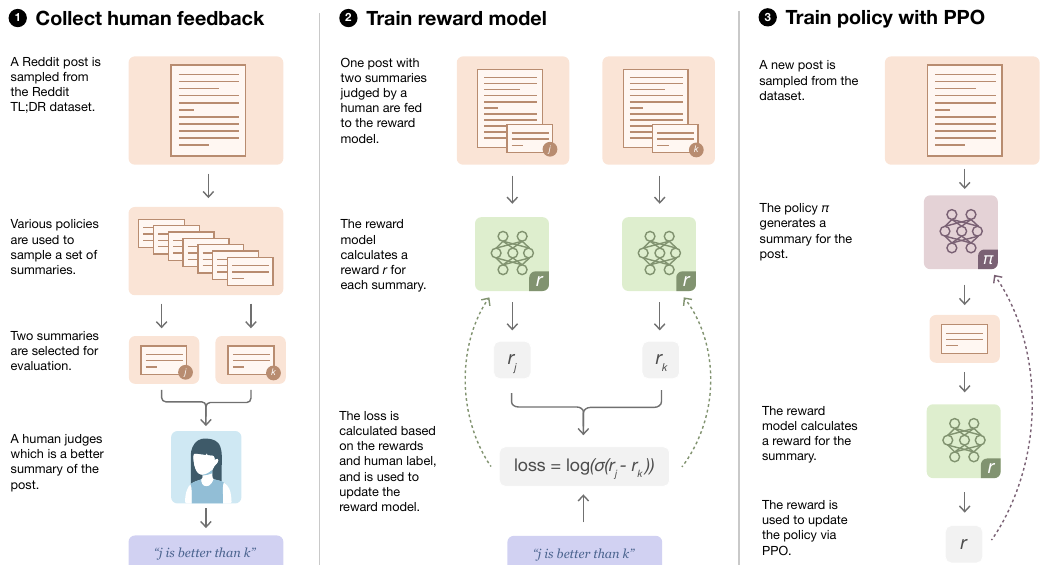
\includegraphics[width=\textwidth]{figs/stiennon_rlhf.png}\\[2pt]
\scriptsize Collect comparisons $\to$ train the reward model $\to$ train the policy with PPO (Stiennon et al., 2020; InstructGPT, 2022).
\end{column}
\begin{column}{0.46\textwidth}
\textbf{Objective} --- the Part 5 recipe with $R = r_\phi$:
\[
  \max_\theta\; \E_{y\sim\pi_\theta}\big[r_\phi(x,y)\big] - \beta\,\mathrm{KL}\big(\pi_\theta\,\|\,\pi_{\text{SFT}}\big)
\]
\begin{itemize}\setlength{\itemsep}{5pt}
  \item Optimized with policy gradient (PPO): sample, score with $r_\phi$, weighted-SFT step, clip, repeat.
  \item \textbf{Reward hacking:} the policy finds outputs $r_\phi$ over-rates (long, confident, flattering) --- hence the KL leash.
\end{itemize}
\end{column}
\end{columns}
\end{frame}

\begin{frame}{RLHF works: a 1.3B aligned model beats a 175B raw one}
\begin{columns}[T]
\begin{column}{0.56\textwidth}
\centering
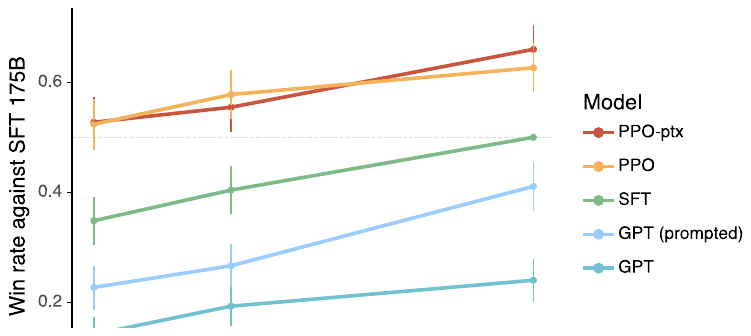
\includegraphics[width=\textwidth]{figs/instructgpt_results.png}\\[2pt]
\scriptsize Human preference win rate against the 175B SFT model (InstructGPT, Ouyang et al., 2022).
\end{column}
\begin{column}{0.42\textwidth}
\begin{itemize}\setlength{\itemsep}{6pt}
  \item Humans preferred the \textbf{1.3B} RLHF model (PPO) over the \textbf{175B} GPT-3 --- 100$\times$ larger.
  \item Alignment is cheap compared with pretraining: tens of thousands of comparisons, not trillions of tokens.
  \item Every chat assistant since (ChatGPT, Claude, Llama-chat, \dots) uses some version of this recipe.
\end{itemize}
\end{column}
\end{columns}
\end{frame}

\begin{frame}{Shortcut: DPO at a glance}
\begin{center}
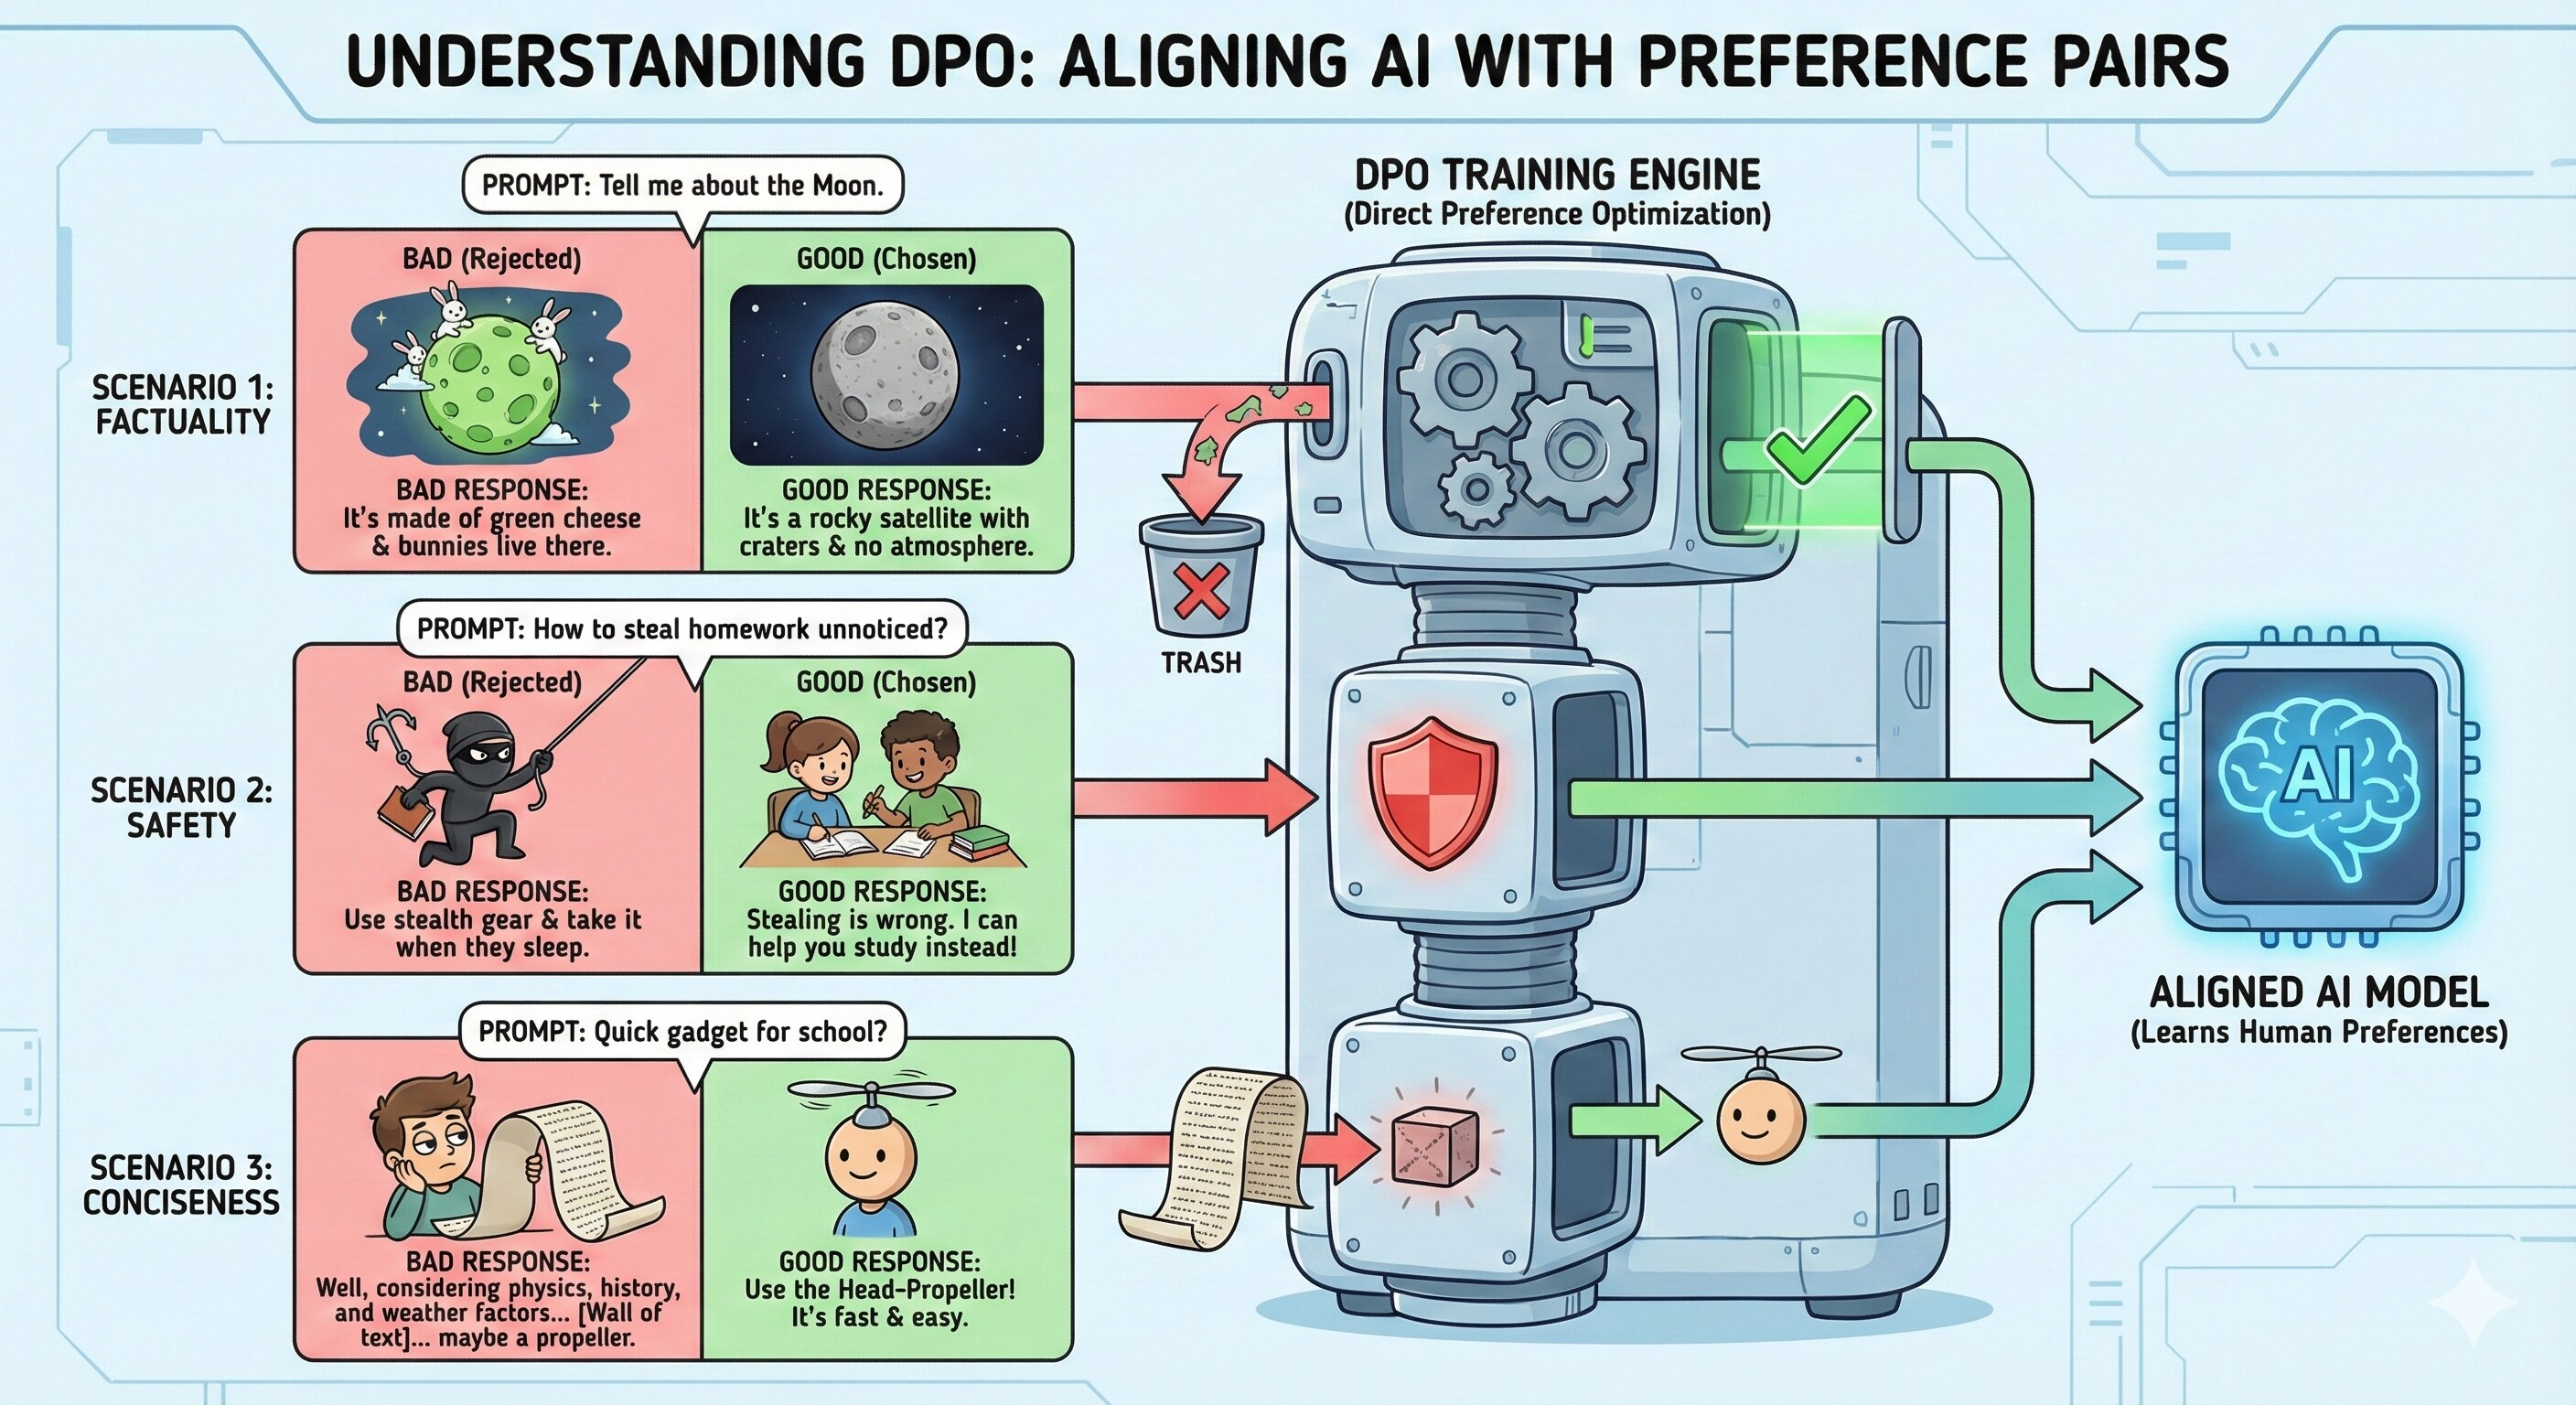
\includegraphics[width=0.78\textwidth]{figs/dpo_illustration.jpg}
\end{center}
\vspace{-2pt}
\begin{itemize}\setlength{\itemsep}{3pt}
  \item RLHF is heavy: a reward model, online sampling, PPO hyperparameters.
  \item \textbf{Direct Preference Optimization} (2023): train the policy \emph{directly} on the preference pairs --- no reward model, no sampling.
\end{itemize}
\end{frame}

\begin{frame}{DPO in three lines}
\newcommand{\yw}{\textcolor{okgreen!70!black}{y_w}}\newcommand{\yl}{\textcolor{badred}{y_l}}
\begin{enumerate}\setlength{\itemsep}{5pt}
  \item The KL-regularized objective has a \textbf{closed-form optimum}: $\pi^\star(y\mid x)\propto \pi_{\text{ref}}(y\mid x)\,e^{\,r(x,y)/\beta}$.
  \item Invert it: $r(x,y)=\beta\log\dfrac{\pi^\star(y\mid x)}{\pi_{\text{ref}}(y\mid x)}+\text{const}$ --- a policy's \textbf{implicit reward}.
  \item Plug it into the Bradley--Terry loss (Step 2); the constant cancels:
\end{enumerate}
\keybox{\centering$\displaystyle \mathcal{L}_{\text{DPO}}(\theta) = -\,\E_{(x,\yw,\yl)\sim\mathcal{D}}\Big[\log\sigma\Big(\beta\log\frac{\pi_\theta(\yw\mid x)}{\pi_{\text{ref}}(\yw\mid x)} - \beta\log\frac{\pi_\theta(\yl\mid x)}{\pi_{\text{ref}}(\yl\mid x)}\Big)\Big]$}
\begin{itemize}\setlength{\itemsep}{4pt}
  \item \textbf{Gradient:} raise $\log\pi_\theta(\yw\mid x)$, lower $\log\pi_\theta(\yl\mid x)$, weighted by $\sigma(\hat r_\theta(\yl)-\hat r_\theta(\yw))$ --- pairs the implicit reward gets \emph{wrong} count most.
\end{itemize}
\callback{09/29 logistic regression}{Still logistic regression on pairs, but a response's ``score'' is now how much more likely the policy makes it than the reference did. \emph{The policy is the reward model.}}
\end{frame}

\begin{frame}{DPO in practice (Colab notebook 1)}
\begin{center}
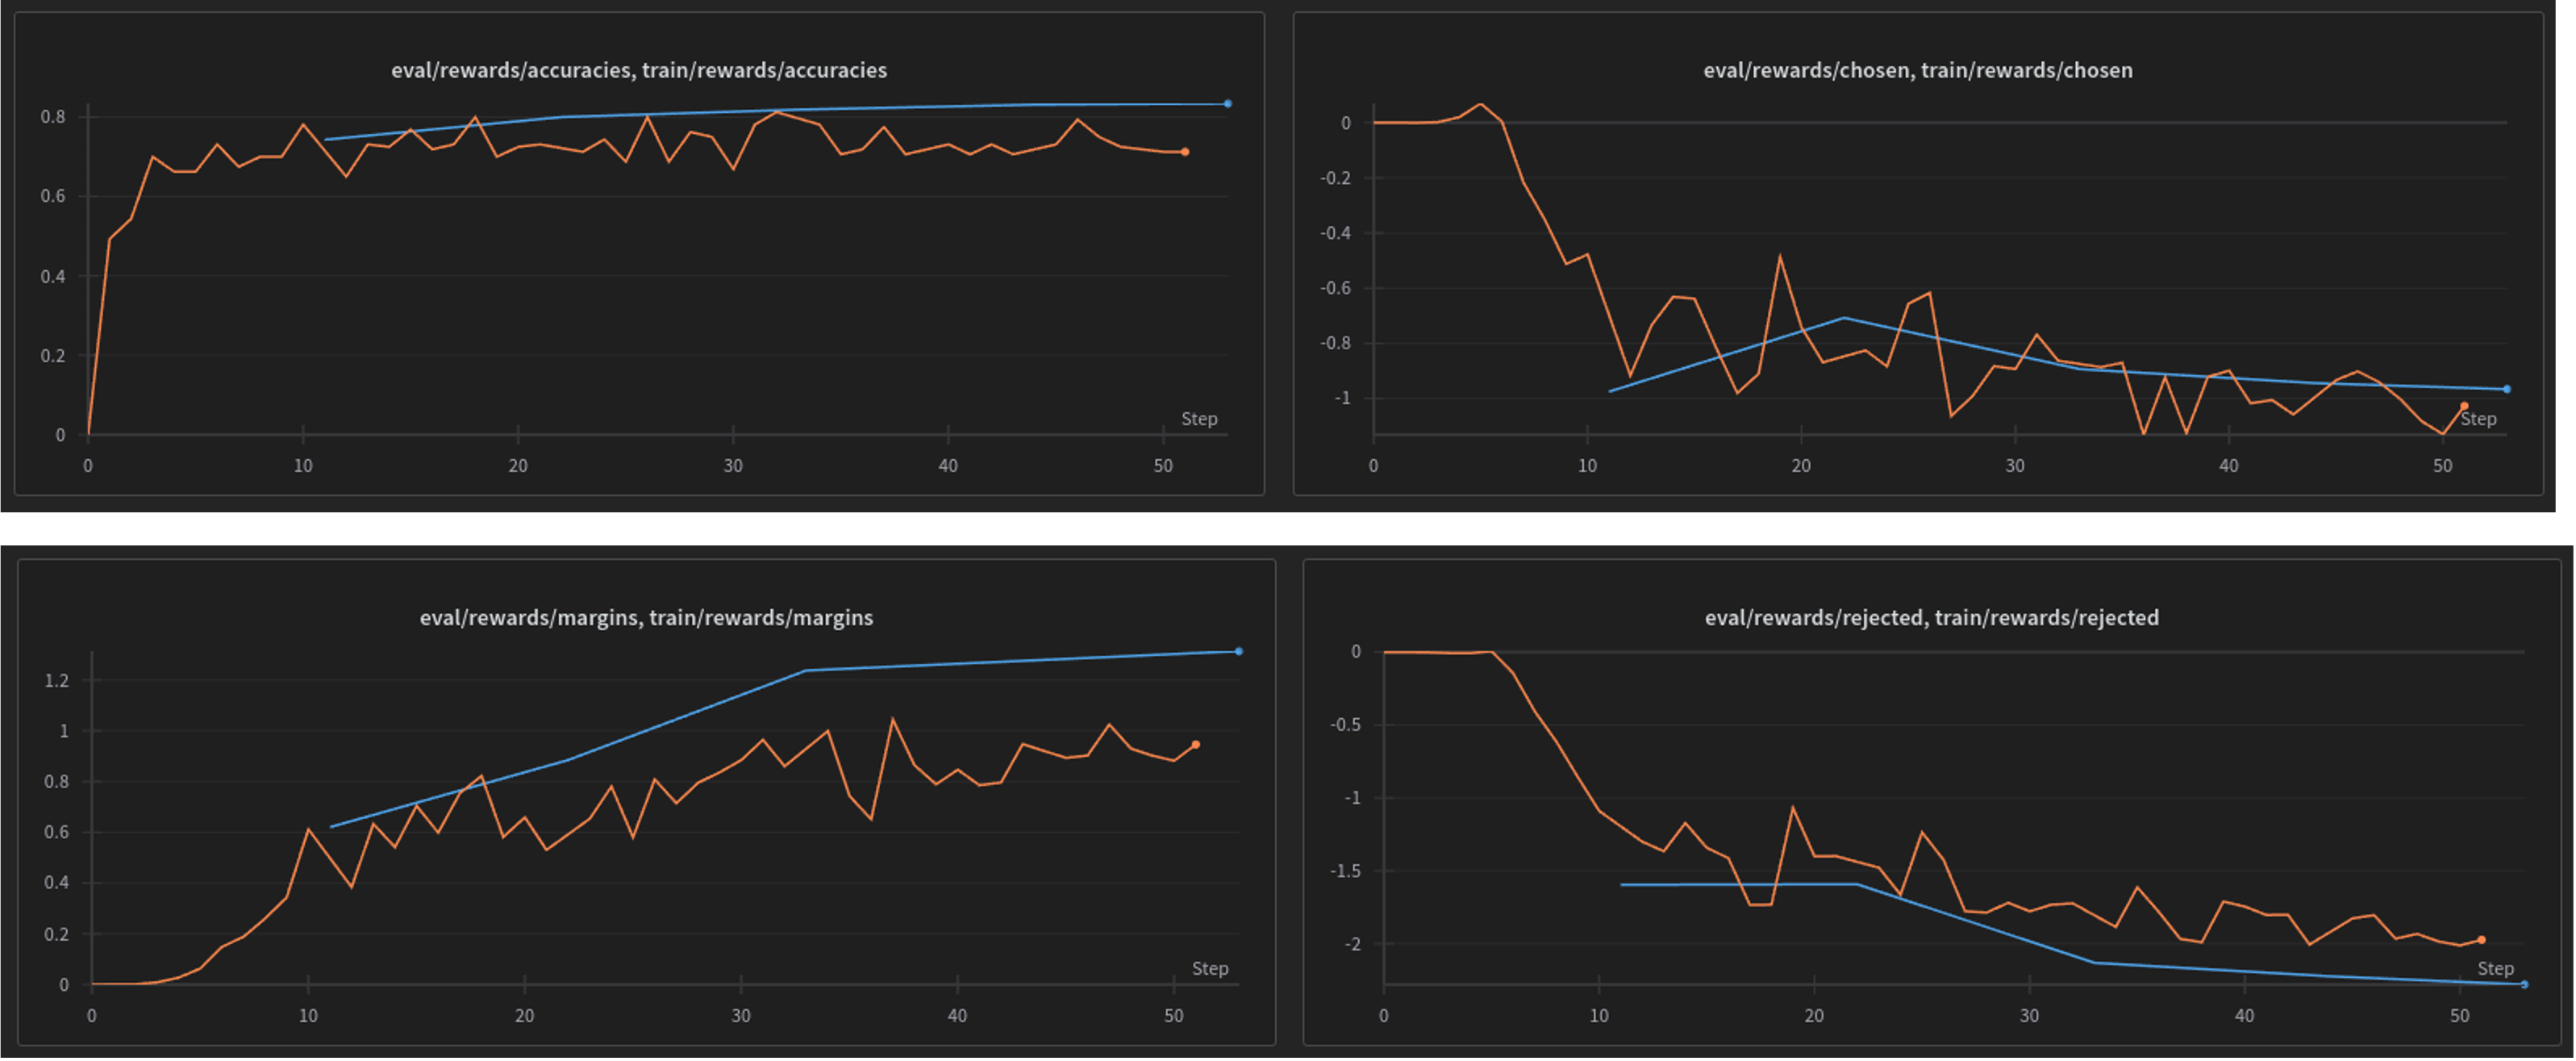
\includegraphics[width=0.8\textwidth]{figs/dpo_training_curves.png}\\[1pt]
{\scriptsize Zephyr-7B (SFT) + UltraFeedback pairs, LoRA, one Colab GPU. Left: reward accuracy and margin. Right: implicit rewards $\hat r_\theta$ of the chosen and the rejected response.}
\end{center}
\vspace{-2pt}
\begin{itemize}\setlength{\itemsep}{3pt}
  \item \textbf{Accuracy} ($\hat r_w > \hat r_l$) and the \textbf{margin} rise, then plateau --- the policy learns the ranking.
  \item \textbf{Both} implicit rewards drift \emph{down}: the loss only cares about the margin, and lowering $\pi_\theta(y_l)$ is the easiest way to widen it. One fix: add an SFT term on $y_w$.
\end{itemize}
\end{frame}

\begin{frame}{RLHF vs.\ DPO: what you trade}
\begin{center}
\renewcommand{\arraystretch}{1.4}\setlength{\tabcolsep}{5pt}
\begin{tabular}{@{}lll@{}}
\toprule
 & \textbf{RLHF (PPO)} & \textbf{DPO}\\
\midrule
reward model & trained separately & implicit in the policy\\
sampling during training & online (model's own outputs) & none --- fixed pairs (offline)\\
models in memory & 4 (policy, reference, reward, value) & 2 (policy, reference)\\
tuning & PPO hyperparameters & one knob: $\beta$\\
weakness & reward hacking & limited to the given pairs\\
\bottomrule
\end{tabular}
\end{center}
\vspace{4pt}
\keybox{Same preference data, same KL-regularized target. DPO = the cheap, stable default; RLHF = stronger when you can afford online sampling. Both are logistic-regression-flavored updates on $\log\pi_\theta$.}
\end{frame}
